% Options for packages loaded elsewhere
% Options for packages loaded elsewhere
\PassOptionsToPackage{unicode}{hyperref}
\PassOptionsToPackage{hyphens}{url}
\PassOptionsToPackage{dvipsnames,svgnames,x11names}{xcolor}
%
\documentclass[
  letterpaper,
  DIV=11,
  numbers=noendperiod]{scrartcl}
\usepackage{xcolor}
\usepackage{amsmath,amssymb}
\setcounter{secnumdepth}{-\maxdimen} % remove section numbering
\usepackage{iftex}
\ifPDFTeX
  \usepackage[T1]{fontenc}
  \usepackage[utf8]{inputenc}
  \usepackage{textcomp} % provide euro and other symbols
\else % if luatex or xetex
  \usepackage{unicode-math} % this also loads fontspec
  \defaultfontfeatures{Scale=MatchLowercase}
  \defaultfontfeatures[\rmfamily]{Ligatures=TeX,Scale=1}
\fi
\usepackage{lmodern}
\ifPDFTeX\else
  % xetex/luatex font selection
\fi
% Use upquote if available, for straight quotes in verbatim environments
\IfFileExists{upquote.sty}{\usepackage{upquote}}{}
\IfFileExists{microtype.sty}{% use microtype if available
  \usepackage[]{microtype}
  \UseMicrotypeSet[protrusion]{basicmath} % disable protrusion for tt fonts
}{}
\makeatletter
\@ifundefined{KOMAClassName}{% if non-KOMA class
  \IfFileExists{parskip.sty}{%
    \usepackage{parskip}
  }{% else
    \setlength{\parindent}{0pt}
    \setlength{\parskip}{6pt plus 2pt minus 1pt}}
}{% if KOMA class
  \KOMAoptions{parskip=half}}
\makeatother
% Make \paragraph and \subparagraph free-standing
\makeatletter
\ifx\paragraph\undefined\else
  \let\oldparagraph\paragraph
  \renewcommand{\paragraph}{
    \@ifstar
      \xxxParagraphStar
      \xxxParagraphNoStar
  }
  \newcommand{\xxxParagraphStar}[1]{\oldparagraph*{#1}\mbox{}}
  \newcommand{\xxxParagraphNoStar}[1]{\oldparagraph{#1}\mbox{}}
\fi
\ifx\subparagraph\undefined\else
  \let\oldsubparagraph\subparagraph
  \renewcommand{\subparagraph}{
    \@ifstar
      \xxxSubParagraphStar
      \xxxSubParagraphNoStar
  }
  \newcommand{\xxxSubParagraphStar}[1]{\oldsubparagraph*{#1}\mbox{}}
  \newcommand{\xxxSubParagraphNoStar}[1]{\oldsubparagraph{#1}\mbox{}}
\fi
\makeatother

\usepackage{color}
\usepackage{fancyvrb}
\newcommand{\VerbBar}{|}
\newcommand{\VERB}{\Verb[commandchars=\\\{\}]}
\DefineVerbatimEnvironment{Highlighting}{Verbatim}{commandchars=\\\{\}}
% Add ',fontsize=\small' for more characters per line
\usepackage{framed}
\definecolor{shadecolor}{RGB}{241,243,245}
\newenvironment{Shaded}{\begin{snugshade}}{\end{snugshade}}
\newcommand{\AlertTok}[1]{\textcolor[rgb]{0.68,0.00,0.00}{#1}}
\newcommand{\AnnotationTok}[1]{\textcolor[rgb]{0.37,0.37,0.37}{#1}}
\newcommand{\AttributeTok}[1]{\textcolor[rgb]{0.40,0.45,0.13}{#1}}
\newcommand{\BaseNTok}[1]{\textcolor[rgb]{0.68,0.00,0.00}{#1}}
\newcommand{\BuiltInTok}[1]{\textcolor[rgb]{0.00,0.23,0.31}{#1}}
\newcommand{\CharTok}[1]{\textcolor[rgb]{0.13,0.47,0.30}{#1}}
\newcommand{\CommentTok}[1]{\textcolor[rgb]{0.37,0.37,0.37}{#1}}
\newcommand{\CommentVarTok}[1]{\textcolor[rgb]{0.37,0.37,0.37}{\textit{#1}}}
\newcommand{\ConstantTok}[1]{\textcolor[rgb]{0.56,0.35,0.01}{#1}}
\newcommand{\ControlFlowTok}[1]{\textcolor[rgb]{0.00,0.23,0.31}{\textbf{#1}}}
\newcommand{\DataTypeTok}[1]{\textcolor[rgb]{0.68,0.00,0.00}{#1}}
\newcommand{\DecValTok}[1]{\textcolor[rgb]{0.68,0.00,0.00}{#1}}
\newcommand{\DocumentationTok}[1]{\textcolor[rgb]{0.37,0.37,0.37}{\textit{#1}}}
\newcommand{\ErrorTok}[1]{\textcolor[rgb]{0.68,0.00,0.00}{#1}}
\newcommand{\ExtensionTok}[1]{\textcolor[rgb]{0.00,0.23,0.31}{#1}}
\newcommand{\FloatTok}[1]{\textcolor[rgb]{0.68,0.00,0.00}{#1}}
\newcommand{\FunctionTok}[1]{\textcolor[rgb]{0.28,0.35,0.67}{#1}}
\newcommand{\ImportTok}[1]{\textcolor[rgb]{0.00,0.46,0.62}{#1}}
\newcommand{\InformationTok}[1]{\textcolor[rgb]{0.37,0.37,0.37}{#1}}
\newcommand{\KeywordTok}[1]{\textcolor[rgb]{0.00,0.23,0.31}{\textbf{#1}}}
\newcommand{\NormalTok}[1]{\textcolor[rgb]{0.00,0.23,0.31}{#1}}
\newcommand{\OperatorTok}[1]{\textcolor[rgb]{0.37,0.37,0.37}{#1}}
\newcommand{\OtherTok}[1]{\textcolor[rgb]{0.00,0.23,0.31}{#1}}
\newcommand{\PreprocessorTok}[1]{\textcolor[rgb]{0.68,0.00,0.00}{#1}}
\newcommand{\RegionMarkerTok}[1]{\textcolor[rgb]{0.00,0.23,0.31}{#1}}
\newcommand{\SpecialCharTok}[1]{\textcolor[rgb]{0.37,0.37,0.37}{#1}}
\newcommand{\SpecialStringTok}[1]{\textcolor[rgb]{0.13,0.47,0.30}{#1}}
\newcommand{\StringTok}[1]{\textcolor[rgb]{0.13,0.47,0.30}{#1}}
\newcommand{\VariableTok}[1]{\textcolor[rgb]{0.07,0.07,0.07}{#1}}
\newcommand{\VerbatimStringTok}[1]{\textcolor[rgb]{0.13,0.47,0.30}{#1}}
\newcommand{\WarningTok}[1]{\textcolor[rgb]{0.37,0.37,0.37}{\textit{#1}}}

\usepackage{longtable,booktabs,array}
\usepackage{calc} % for calculating minipage widths
% Correct order of tables after \paragraph or \subparagraph
\usepackage{etoolbox}
\makeatletter
\patchcmd\longtable{\par}{\if@noskipsec\mbox{}\fi\par}{}{}
\makeatother
% Allow footnotes in longtable head/foot
\IfFileExists{footnotehyper.sty}{\usepackage{footnotehyper}}{\usepackage{footnote}}
\makesavenoteenv{longtable}
\usepackage{graphicx}
\makeatletter
\newsavebox\pandoc@box
\newcommand*\pandocbounded[1]{% scales image to fit in text height/width
  \sbox\pandoc@box{#1}%
  \Gscale@div\@tempa{\textheight}{\dimexpr\ht\pandoc@box+\dp\pandoc@box\relax}%
  \Gscale@div\@tempb{\linewidth}{\wd\pandoc@box}%
  \ifdim\@tempb\p@<\@tempa\p@\let\@tempa\@tempb\fi% select the smaller of both
  \ifdim\@tempa\p@<\p@\scalebox{\@tempa}{\usebox\pandoc@box}%
  \else\usebox{\pandoc@box}%
  \fi%
}
% Set default figure placement to htbp
\def\fps@figure{htbp}
\makeatother





\setlength{\emergencystretch}{3em} % prevent overfull lines

\providecommand{\tightlist}{%
  \setlength{\itemsep}{0pt}\setlength{\parskip}{0pt}}



 


\KOMAoption{captions}{tableheading}
\makeatletter
\@ifpackageloaded{caption}{}{\usepackage{caption}}
\AtBeginDocument{%
\ifdefined\contentsname
  \renewcommand*\contentsname{Table of contents}
\else
  \newcommand\contentsname{Table of contents}
\fi
\ifdefined\listfigurename
  \renewcommand*\listfigurename{List of Figures}
\else
  \newcommand\listfigurename{List of Figures}
\fi
\ifdefined\listtablename
  \renewcommand*\listtablename{List of Tables}
\else
  \newcommand\listtablename{List of Tables}
\fi
\ifdefined\figurename
  \renewcommand*\figurename{Figure}
\else
  \newcommand\figurename{Figure}
\fi
\ifdefined\tablename
  \renewcommand*\tablename{Table}
\else
  \newcommand\tablename{Table}
\fi
}
\@ifpackageloaded{float}{}{\usepackage{float}}
\floatstyle{ruled}
\@ifundefined{c@chapter}{\newfloat{codelisting}{h}{lop}}{\newfloat{codelisting}{h}{lop}[chapter]}
\floatname{codelisting}{Listing}
\newcommand*\listoflistings{\listof{codelisting}{List of Listings}}
\makeatother
\makeatletter
\makeatother
\makeatletter
\@ifpackageloaded{caption}{}{\usepackage{caption}}
\@ifpackageloaded{subcaption}{}{\usepackage{subcaption}}
\makeatother
\usepackage{bookmark}
\IfFileExists{xurl.sty}{\usepackage{xurl}}{} % add URL line breaks if available
\urlstyle{same}
\hypersetup{
  pdfauthor={Pranav},
  colorlinks=true,
  linkcolor={blue},
  filecolor={Maroon},
  citecolor={Blue},
  urlcolor={Blue},
  pdfcreator={LaTeX via pandoc}}


\author{Pranav}
\date{}
\begin{document}


\textbf{ED 6002: Optimization Methods in Engineering Design (2025-26)}

\emph{Assignment 1 \textbar{} Pranav D \textbar{} ns26z167}

\subsection{At a Glance}\label{at-a-glance}

\begin{itemize}
\tightlist
\item
  Created a 2m beam with the specified I cross section
\item
  Applied 9810 N load on the top face
\item
  Simulated for the exhaustive set of parameteric configurations
\item
  3 levels \^{} 6 parameters results in 729 models!
\end{itemize}

\pandocbounded{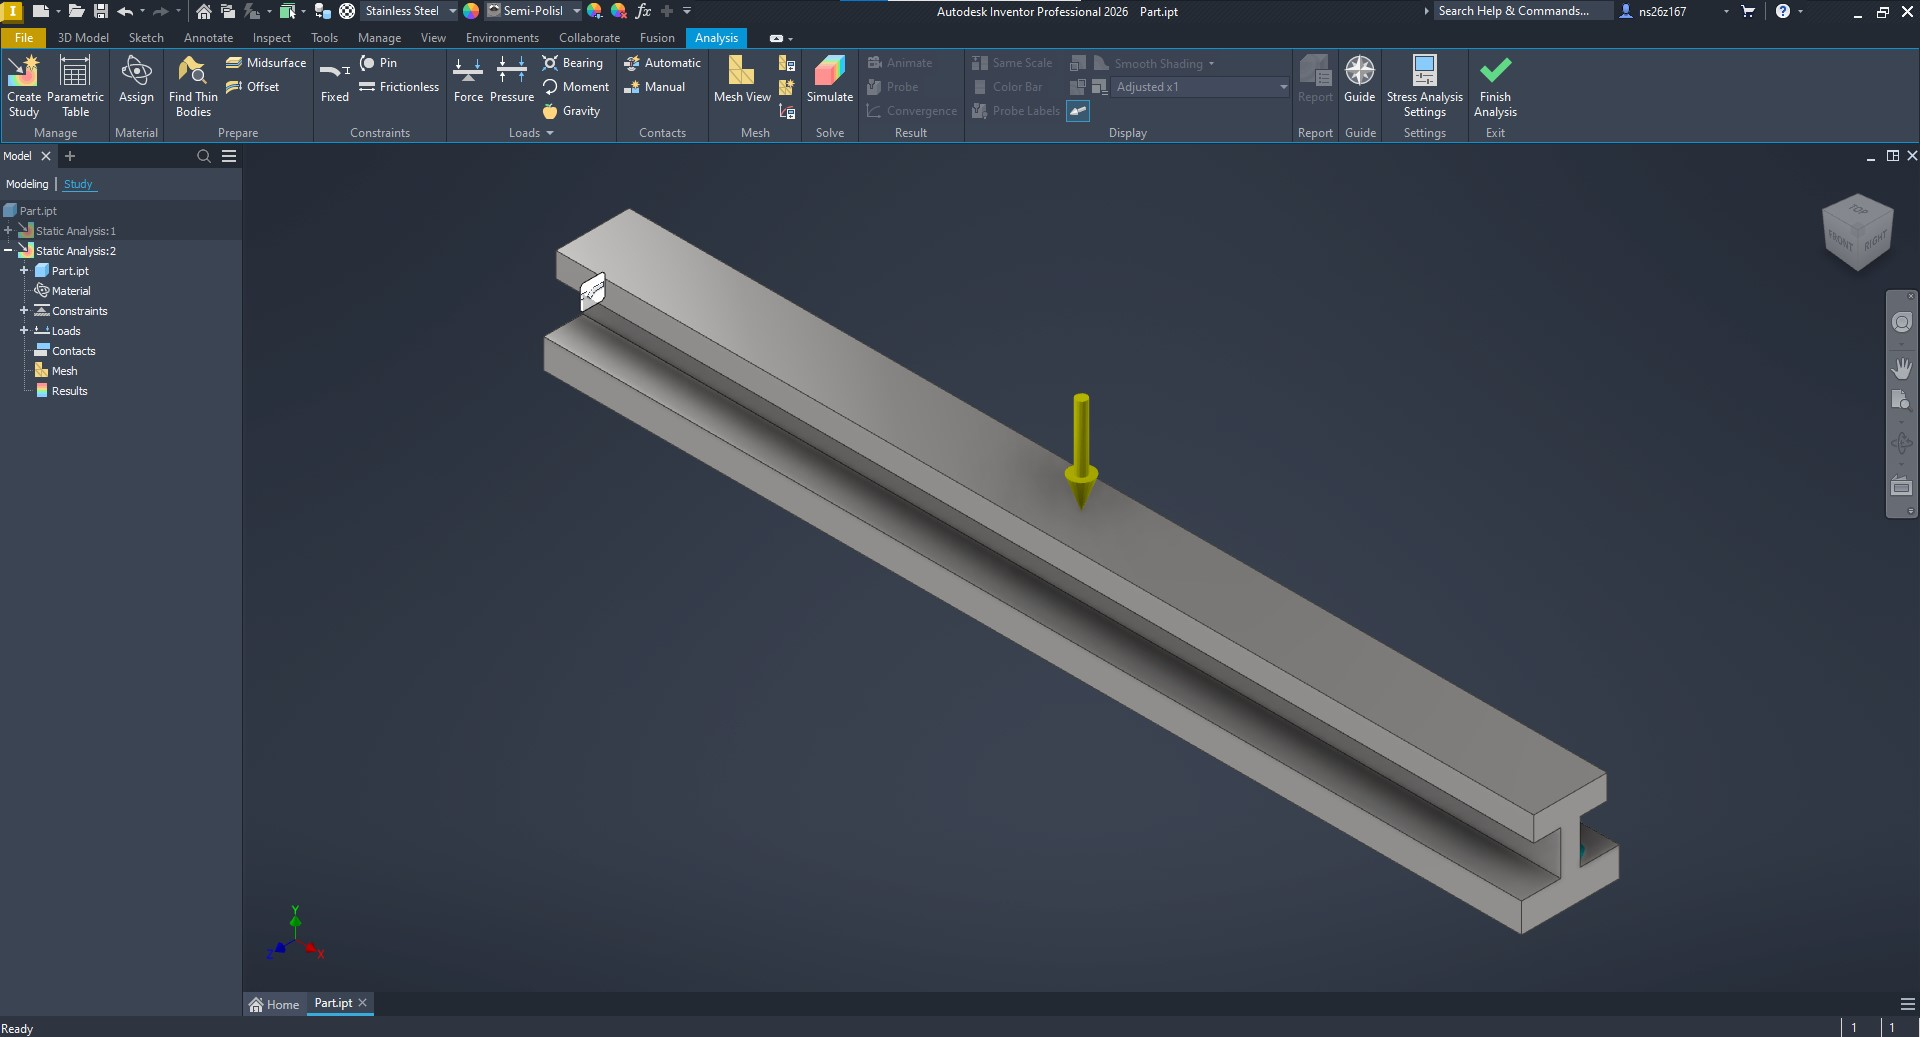
\includegraphics[keepaspectratio]{bar.jpg}}

\subsection{Q1. Sensitivity of each variable on
outcomes}\label{q1.-sensitivity-of-each-variable-on-outcomes}

\begin{itemize}
\tightlist
\item
  To analyse the senstivity of a each variable in the cross section
  dimension, I chose to go by OFAT \emph{(One Factor at a Time)}
  approach.
\item
  Change one variable, keep everything else the same (base dimensions),
  and analyse the trends in outcomes.
\end{itemize}

\subsection{}\label{section}

\subsubsection{Sensitivity plot}\label{sensitivity-plot}

\pandocbounded{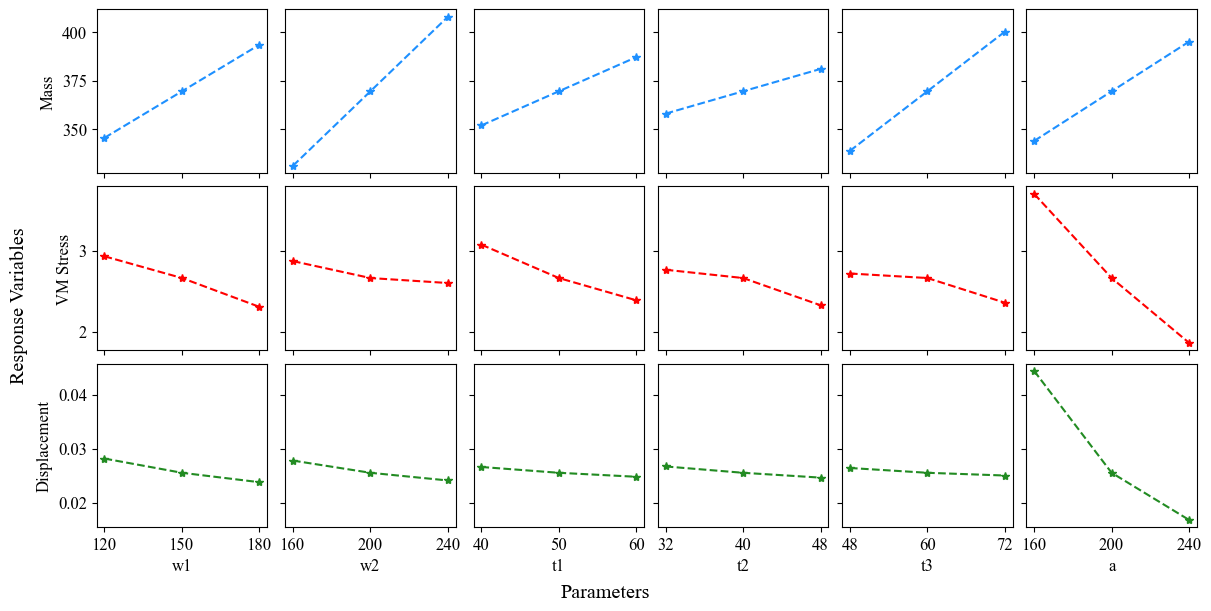
\includegraphics[keepaspectratio]{plot1.png}}

\subsection{Comments}\label{comments}

\begin{itemize}
\tightlist
\item
  Mass is directly proportional to all the parameters -- Greater the
  cross section, greater the mass.
\item
  Though Mass is sensitive to all the parameters, its strongly
  influenced by \textbf{\emph{w2}}.
\item
  VM stress decrease as size increases, with \textbf{\emph{a}}
  contributing for significant reduction compared to others.
\item
  Similarly displacement also decreases with increase in cross section
  parameters, but again \textbf{\emph{a}} have higher effect.
\end{itemize}

\subsection{Q2. Optima based on DoE}\label{q2.-optima-based-on-doe}

\paragraph{Objective Function:}\label{objective-function}

\[
Minimize: Mass(p)
\]

\paragraph{Design Space:}\label{design-space}

\[
p \in [0.8 p_0, 1.2 p_0]\\
p \in {w1,w2,t1,t2,t3,a}\\
p_0 := \text{nominal value of }p
\]

\paragraph{Constraints:}\label{constraints}

\[
\delta(p) \le 2~\text{mm}, \quad \text{FOS}(p) \ge 1.5
\]

\subsection{}\label{section-1}

\subsubsection{Optima}\label{optima}

\begin{longtable}[]{@{}llll@{}}
\toprule\noalign{}
Parameter & Value (mm) & Parameter & Value (mm) \\
\midrule\noalign{}
\endhead
\bottomrule\noalign{}
\endlastfoot
w1 & 120 & t1 & 40 \\
w2 & 160 & t2 & 32 \\
a & 160 & t3 & 48 \\
\end{longtable}

\[
\begin{align}
\text{Mass} &= 236.54 \text{ kg}\\
\delta &= 0.058 \text{ mm} \\
\text{Max VM Stress} &= 5.1 \text{ MPa}\\
\end{align}
\]

\subsection{Q3. Polynomial response
surface}\label{q3.-polynomial-response-surface}

\pandocbounded{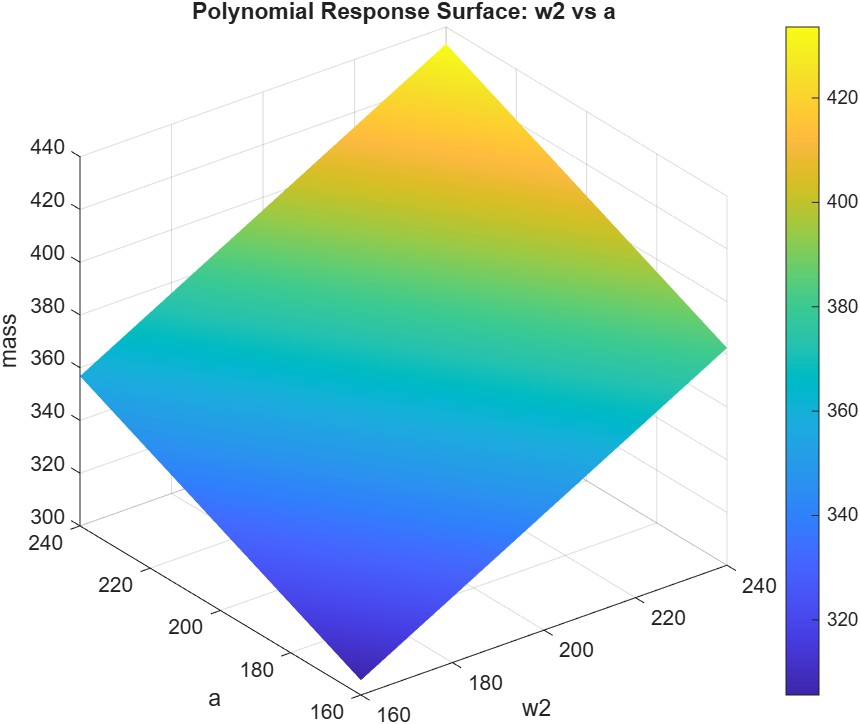
\includegraphics[keepaspectratio]{plot2.jpg}}

\subsection{Code}\label{code}

\begin{Shaded}
\begin{Highlighting}[]
\VariableTok{data} \OperatorTok{=} \VariableTok{readtable}\NormalTok{(}\SpecialStringTok{\textquotesingle{}master.csv\textquotesingle{}}\NormalTok{)}\OperatorTok{;}

\VariableTok{X} \OperatorTok{=} \VariableTok{data}\NormalTok{\{}\OperatorTok{:,}\NormalTok{ \{}\SpecialStringTok{\textquotesingle{}w1\textquotesingle{}}\OperatorTok{,}\SpecialStringTok{\textquotesingle{}w2\textquotesingle{}}\OperatorTok{,}\SpecialStringTok{\textquotesingle{}t1\textquotesingle{}}\OperatorTok{,}\SpecialStringTok{\textquotesingle{}t2\textquotesingle{}}\OperatorTok{,}\SpecialStringTok{\textquotesingle{}t3\textquotesingle{}}\OperatorTok{,}\SpecialStringTok{\textquotesingle{}a\textquotesingle{}}\NormalTok{\}\}}\OperatorTok{;}
\VariableTok{y} \OperatorTok{=} \VariableTok{data}\NormalTok{.}\VariableTok{mass}\OperatorTok{;}

\VariableTok{tbl} \OperatorTok{=} \VariableTok{data}\NormalTok{(}\OperatorTok{:,}\NormalTok{ \{}\SpecialStringTok{\textquotesingle{}w1\textquotesingle{}}\OperatorTok{,}\SpecialStringTok{\textquotesingle{}w2\textquotesingle{}}\OperatorTok{,}\SpecialStringTok{\textquotesingle{}t1\textquotesingle{}}\OperatorTok{,}\SpecialStringTok{\textquotesingle{}t2\textquotesingle{}}\OperatorTok{,}\SpecialStringTok{\textquotesingle{}t3\textquotesingle{}}\OperatorTok{,}\SpecialStringTok{\textquotesingle{}a\textquotesingle{}}\OperatorTok{,}\SpecialStringTok{\textquotesingle{}mass\textquotesingle{}}\NormalTok{\})}\OperatorTok{;}

\VariableTok{model} \OperatorTok{=} \VariableTok{fitlm}\NormalTok{(}\VariableTok{tbl}\OperatorTok{,} \SpecialStringTok{\textquotesingle{}quadratic\textquotesingle{}}\NormalTok{)}\OperatorTok{;}

\VariableTok{disp}\NormalTok{(}\VariableTok{model}\NormalTok{)}

\VariableTok{model}\NormalTok{.}\VariableTok{Rsquared}

\NormalTok{[}\VariableTok{w2Grid}\OperatorTok{,} \VariableTok{aGrid}\NormalTok{] }\OperatorTok{=} \VariableTok{meshgrid}\NormalTok{( }\OperatorTok{...}
    \VariableTok{linspace}\NormalTok{(}\VariableTok{min}\NormalTok{(}\VariableTok{data}\NormalTok{.}\VariableTok{w2}\NormalTok{)}\OperatorTok{,} \VariableTok{max}\NormalTok{(}\VariableTok{data}\NormalTok{.}\VariableTok{w2}\NormalTok{)}\OperatorTok{,} \FloatTok{50}\NormalTok{)}\OperatorTok{,} \OperatorTok{...}
    \VariableTok{linspace}\NormalTok{(}\VariableTok{min}\NormalTok{(}\VariableTok{data}\NormalTok{.}\VariableTok{a}\NormalTok{)}\OperatorTok{,}  \VariableTok{max}\NormalTok{(}\VariableTok{data}\NormalTok{.}\VariableTok{a}\NormalTok{)}\OperatorTok{,}  \FloatTok{50}\NormalTok{))}\OperatorTok{;}

\VariableTok{w1} \OperatorTok{=} \VariableTok{mean}\NormalTok{(}\VariableTok{data}\NormalTok{.}\VariableTok{w1}\NormalTok{)}\OperatorTok{;}
\VariableTok{t1} \OperatorTok{=} \VariableTok{mean}\NormalTok{(}\VariableTok{data}\NormalTok{.}\VariableTok{t1}\NormalTok{)}\OperatorTok{;}
\VariableTok{t2} \OperatorTok{=} \VariableTok{mean}\NormalTok{(}\VariableTok{data}\NormalTok{.}\VariableTok{t2}\NormalTok{)}\OperatorTok{;}
\VariableTok{t3} \OperatorTok{=} \VariableTok{mean}\NormalTok{(}\VariableTok{data}\NormalTok{.}\VariableTok{t3}\NormalTok{)}\OperatorTok{;}

\VariableTok{gridTable} \OperatorTok{=} \VariableTok{table}\NormalTok{( }\OperatorTok{...}
    \VariableTok{repmat}\NormalTok{(}\VariableTok{w1}\OperatorTok{,} \VariableTok{numel}\NormalTok{(}\VariableTok{w2Grid}\NormalTok{)}\OperatorTok{,} \FloatTok{1}\NormalTok{)}\OperatorTok{,} \OperatorTok{...}
    \VariableTok{w2Grid}\NormalTok{(}\OperatorTok{:}\NormalTok{)}\OperatorTok{,} \OperatorTok{...}
    \VariableTok{repmat}\NormalTok{(}\VariableTok{t1}\OperatorTok{,} \VariableTok{numel}\NormalTok{(}\VariableTok{w2Grid}\NormalTok{)}\OperatorTok{,} \FloatTok{1}\NormalTok{)}\OperatorTok{,} \OperatorTok{...}
    \VariableTok{repmat}\NormalTok{(}\VariableTok{t2}\OperatorTok{,} \VariableTok{numel}\NormalTok{(}\VariableTok{w2Grid}\NormalTok{)}\OperatorTok{,} \FloatTok{1}\NormalTok{)}\OperatorTok{,} \OperatorTok{...}
    \VariableTok{repmat}\NormalTok{(}\VariableTok{t3}\OperatorTok{,} \VariableTok{numel}\NormalTok{(}\VariableTok{w2Grid}\NormalTok{)}\OperatorTok{,} \FloatTok{1}\NormalTok{)}\OperatorTok{,} \OperatorTok{...}
    \VariableTok{aGrid}\NormalTok{(}\OperatorTok{:}\NormalTok{)}\OperatorTok{,} \OperatorTok{...}
    \SpecialStringTok{\textquotesingle{}VariableNames\textquotesingle{}}\OperatorTok{,}\NormalTok{ \{}\SpecialStringTok{\textquotesingle{}w1\textquotesingle{}}\OperatorTok{,}\SpecialStringTok{\textquotesingle{}w2\textquotesingle{}}\OperatorTok{,}\SpecialStringTok{\textquotesingle{}t1\textquotesingle{}}\OperatorTok{,}\SpecialStringTok{\textquotesingle{}t2\textquotesingle{}}\OperatorTok{,}\SpecialStringTok{\textquotesingle{}t3\textquotesingle{}}\OperatorTok{,}\SpecialStringTok{\textquotesingle{}a\textquotesingle{}}\NormalTok{\})}\OperatorTok{;}

\VariableTok{massPred} \OperatorTok{=} \VariableTok{predict}\NormalTok{(}\VariableTok{model}\OperatorTok{,} \VariableTok{gridTable}\NormalTok{)}\OperatorTok{;}

\VariableTok{massSurface} \OperatorTok{=} \VariableTok{reshape}\NormalTok{(}\VariableTok{massPred}\OperatorTok{,} \VariableTok{size}\NormalTok{(}\VariableTok{w2Grid}\NormalTok{))}\OperatorTok{;}

\VariableTok{surf}\NormalTok{(}\VariableTok{w2Grid}\OperatorTok{,} \VariableTok{aGrid}\OperatorTok{,} \VariableTok{massSurface}\NormalTok{)}
\VariableTok{xlabel}\NormalTok{(}\SpecialStringTok{\textquotesingle{}w2\textquotesingle{}}\NormalTok{)}
\VariableTok{ylabel}\NormalTok{(}\SpecialStringTok{\textquotesingle{}a\textquotesingle{}}\NormalTok{)}
\VariableTok{zlabel}\NormalTok{(}\SpecialStringTok{\textquotesingle{}mass\textquotesingle{}}\NormalTok{)}
\VariableTok{title}\NormalTok{(}\SpecialStringTok{\textquotesingle{}Polynomial Response Surface: w2 vs a\textquotesingle{}}\NormalTok{)}
\VariableTok{colorbar}
\VariableTok{shading} \VariableTok{interp}
\end{Highlighting}
\end{Shaded}

\subsection{\texorpdfstring{Q4. Optima using \textbf{\emph{fmincon}} -
Code}{Q4. Optima using fmincon - Code}}\label{q4.-optima-using-fmincon---code}

\begin{Shaded}
\begin{Highlighting}[]

\VariableTok{data} \OperatorTok{=} \VariableTok{readtable}\NormalTok{(}\SpecialStringTok{\textquotesingle{}master.csv\textquotesingle{}}\NormalTok{)}\OperatorTok{;}
\VariableTok{predictorNames} \OperatorTok{=}\NormalTok{ \{}\SpecialStringTok{\textquotesingle{}w1\textquotesingle{}}\OperatorTok{,} \SpecialStringTok{\textquotesingle{}w2\textquotesingle{}}\OperatorTok{,} \SpecialStringTok{\textquotesingle{}t1\textquotesingle{}}\OperatorTok{,} \SpecialStringTok{\textquotesingle{}t2\textquotesingle{}}\OperatorTok{,} \SpecialStringTok{\textquotesingle{}t3\textquotesingle{}}\OperatorTok{,} \SpecialStringTok{\textquotesingle{}a\textquotesingle{}}\NormalTok{\}}\OperatorTok{;}
\VariableTok{responseName}   \OperatorTok{=} \SpecialStringTok{\textquotesingle{}mass\textquotesingle{}}\OperatorTok{;}
\VariableTok{tbl} \OperatorTok{=} \VariableTok{data}\NormalTok{(}\OperatorTok{:,}\NormalTok{ [}\VariableTok{predictorNames}\OperatorTok{,}\NormalTok{ \{}\VariableTok{responseName}\NormalTok{\}])}\OperatorTok{;}
\VariableTok{model} \OperatorTok{=} \VariableTok{fitlm}\NormalTok{(}\VariableTok{tbl}\OperatorTok{,} \SpecialStringTok{\textquotesingle{}quadratic\textquotesingle{}}\NormalTok{)}\OperatorTok{;}
\VariableTok{fprintf}\NormalTok{(}\SpecialStringTok{\textquotesingle{}\textbackslash{}n================ MODEL SUMMARY ================\textbackslash{}n\textquotesingle{}}\NormalTok{)}\OperatorTok{;}
\VariableTok{disp}\NormalTok{(}\VariableTok{model}\NormalTok{)}\OperatorTok{;}
\VariableTok{fprintf}\NormalTok{(}\SpecialStringTok{\textquotesingle{}R{-}squared: \%.4f\textbackslash{}n\textquotesingle{}}\OperatorTok{,} \VariableTok{model}\NormalTok{.}\VariableTok{Rsquared}\NormalTok{.}\VariableTok{Ordinary}\NormalTok{)}\OperatorTok{;}
\VariableTok{objFun} \OperatorTok{=} \OperatorTok{@}\NormalTok{(}\VariableTok{x}\NormalTok{) }\VariableTok{predict}\NormalTok{(}\VariableTok{model}\OperatorTok{,} \VariableTok{array2table}\NormalTok{(}\VariableTok{x}\OperatorTok{,} \SpecialStringTok{\textquotesingle{}VariableNames\textquotesingle{}}\OperatorTok{,} \VariableTok{predictorNames}\NormalTok{))}\OperatorTok{;}
\VariableTok{lb} \OperatorTok{=}\NormalTok{ [}\VariableTok{min}\NormalTok{(}\VariableTok{data}\NormalTok{.}\VariableTok{w1}\NormalTok{)}\OperatorTok{,} \VariableTok{min}\NormalTok{(}\VariableTok{data}\NormalTok{.}\VariableTok{w2}\NormalTok{)}\OperatorTok{,} \VariableTok{min}\NormalTok{(}\VariableTok{data}\NormalTok{.}\VariableTok{t1}\NormalTok{)}\OperatorTok{,} \OperatorTok{...}
      \VariableTok{min}\NormalTok{(}\VariableTok{data}\NormalTok{.}\VariableTok{t2}\NormalTok{)}\OperatorTok{,} \VariableTok{min}\NormalTok{(}\VariableTok{data}\NormalTok{.}\VariableTok{t3}\NormalTok{)}\OperatorTok{,} \VariableTok{min}\NormalTok{(}\VariableTok{data}\NormalTok{.}\VariableTok{a}\NormalTok{)]}\OperatorTok{;}
\VariableTok{ub} \OperatorTok{=}\NormalTok{ [}\VariableTok{max}\NormalTok{(}\VariableTok{data}\NormalTok{.}\VariableTok{w1}\NormalTok{)}\OperatorTok{,} \VariableTok{max}\NormalTok{(}\VariableTok{data}\NormalTok{.}\VariableTok{w2}\NormalTok{)}\OperatorTok{,} \VariableTok{max}\NormalTok{(}\VariableTok{data}\NormalTok{.}\VariableTok{t1}\NormalTok{)}\OperatorTok{,} \OperatorTok{...}
      \VariableTok{max}\NormalTok{(}\VariableTok{data}\NormalTok{.}\VariableTok{t2}\NormalTok{)}\OperatorTok{,} \VariableTok{max}\NormalTok{(}\VariableTok{data}\NormalTok{.}\VariableTok{t3}\NormalTok{)}\OperatorTok{,} \VariableTok{max}\NormalTok{(}\VariableTok{data}\NormalTok{.}\VariableTok{a}\NormalTok{)]}\OperatorTok{;}
\VariableTok{x0} \OperatorTok{=}\NormalTok{ (}\VariableTok{lb} \OperatorTok{+} \VariableTok{ub}\NormalTok{) }\OperatorTok{/} \FloatTok{2}\OperatorTok{;}
\VariableTok{limit} \OperatorTok{=}\NormalTok{ (}\VariableTok{mean}\NormalTok{(}\VariableTok{data}\NormalTok{.}\VariableTok{t1}\NormalTok{) }\OperatorTok{+} \VariableTok{mean}\NormalTok{(}\VariableTok{data}\NormalTok{.}\VariableTok{t2}\NormalTok{)) }\OperatorTok{*} \FloatTok{1.5}\OperatorTok{;}
\VariableTok{nonlcon} \OperatorTok{=} \OperatorTok{@}\NormalTok{(}\VariableTok{x}\NormalTok{) }\VariableTok{deal}\NormalTok{(}\VariableTok{x}\NormalTok{(}\FloatTok{3}\NormalTok{) }\OperatorTok{+} \VariableTok{x}\NormalTok{(}\FloatTok{4}\NormalTok{) }\OperatorTok{{-}} \VariableTok{limit}\OperatorTok{,}\NormalTok{ [])}\OperatorTok{;} 
\VariableTok{options} \OperatorTok{=} \VariableTok{optimoptions}\NormalTok{(}\SpecialStringTok{\textquotesingle{}fmincon\textquotesingle{}}\OperatorTok{,} \OperatorTok{...}
    \SpecialStringTok{\textquotesingle{}Algorithm\textquotesingle{}}\OperatorTok{,} \SpecialStringTok{\textquotesingle{}sqp\textquotesingle{}}\OperatorTok{,} \OperatorTok{...}
    \SpecialStringTok{\textquotesingle{}Display\textquotesingle{}}\OperatorTok{,} \SpecialStringTok{\textquotesingle{}iter\textquotesingle{}}\OperatorTok{,} \OperatorTok{...}
    \SpecialStringTok{\textquotesingle{}MaxFunctionEvaluations\textquotesingle{}}\OperatorTok{,} \FloatTok{5000}\OperatorTok{,} \OperatorTok{...}
    \SpecialStringTok{\textquotesingle{}ConstraintTolerance\textquotesingle{}}\OperatorTok{,} \FloatTok{1e{-}9}\OperatorTok{,} \OperatorTok{...}
    \SpecialStringTok{\textquotesingle{}OptimalityTolerance\textquotesingle{}}\OperatorTok{,} \FloatTok{1e{-}9}\OperatorTok{,} \OperatorTok{...}
    \SpecialStringTok{\textquotesingle{}StepTolerance\textquotesingle{}}\OperatorTok{,} \FloatTok{1e{-}10}\NormalTok{)}\OperatorTok{;}
\NormalTok{[}\VariableTok{x\_opt}\OperatorTok{,} \VariableTok{fval\_opt}\NormalTok{] }\OperatorTok{=} \VariableTok{fmincon}\NormalTok{(}\VariableTok{objFun}\OperatorTok{,} \VariableTok{x0}\OperatorTok{,} \OperatorTok{...}
\NormalTok{                            []}\OperatorTok{,}\NormalTok{ []}\OperatorTok{,} \OperatorTok{...}     
\NormalTok{                            []}\OperatorTok{,}\NormalTok{ []}\OperatorTok{,} \OperatorTok{...}     
                            \VariableTok{lb}\OperatorTok{,} \VariableTok{ub}\OperatorTok{,} \OperatorTok{...}     
                            \VariableTok{nonlcon}\OperatorTok{,} \OperatorTok{...}    
                            \VariableTok{options}\NormalTok{)}\OperatorTok{;}
\VariableTok{problem} \OperatorTok{=} \VariableTok{createOptimProblem}\NormalTok{(}\SpecialStringTok{\textquotesingle{}fmincon\textquotesingle{}}\OperatorTok{,} \OperatorTok{...}
    \SpecialStringTok{\textquotesingle{}objective\textquotesingle{}}\OperatorTok{,} \VariableTok{objFun}\OperatorTok{,} \OperatorTok{...}
    \SpecialStringTok{\textquotesingle{}x0\textquotesingle{}}\OperatorTok{,} \VariableTok{x0}\OperatorTok{,} \OperatorTok{...}
    \SpecialStringTok{\textquotesingle{}lb\textquotesingle{}}\OperatorTok{,} \VariableTok{lb}\OperatorTok{,} \SpecialStringTok{\textquotesingle{}ub\textquotesingle{}}\OperatorTok{,} \VariableTok{ub}\OperatorTok{,} \OperatorTok{...}
    \SpecialStringTok{\textquotesingle{}nonlcon\textquotesingle{}}\OperatorTok{,} \VariableTok{nonlcon}\OperatorTok{,} \OperatorTok{...}
    \SpecialStringTok{\textquotesingle{}options\textquotesingle{}}\OperatorTok{,} \VariableTok{options}\NormalTok{)}\OperatorTok{;}
\VariableTok{ms} \OperatorTok{=} \VariableTok{MultiStart}\NormalTok{(}\SpecialStringTok{\textquotesingle{}Display\textquotesingle{}}\OperatorTok{,} \SpecialStringTok{\textquotesingle{}off\textquotesingle{}}\NormalTok{)}\OperatorTok{;}
\NormalTok{[}\VariableTok{x\_global}\OperatorTok{,} \VariableTok{fval\_global}\NormalTok{] }\OperatorTok{=} \VariableTok{run}\NormalTok{(}\VariableTok{ms}\OperatorTok{,} \VariableTok{problem}\OperatorTok{,} \FloatTok{1}\NormalTok{)}\OperatorTok{;}
\VariableTok{fprintf}\NormalTok{(}\SpecialStringTok{\textquotesingle{}\textbackslash{}n================ LOCAL OPTIMUM (fmincon) ================\textbackslash{}n\textquotesingle{}}\NormalTok{)}\OperatorTok{;}
\VariableTok{disp}\NormalTok{(}\VariableTok{array2table}\NormalTok{(}\VariableTok{x\_opt}\OperatorTok{,} \SpecialStringTok{\textquotesingle{}VariableNames\textquotesingle{}}\OperatorTok{,} \VariableTok{predictorNames}\NormalTok{))}\OperatorTok{;}
\VariableTok{fprintf}\NormalTok{(}\SpecialStringTok{\textquotesingle{}Minimum mass (local) = \%.4f\textbackslash{}n\textquotesingle{}}\OperatorTok{,} \VariableTok{fval\_opt}\NormalTok{)}\OperatorTok{;}
\VariableTok{fprintf}\NormalTok{(}\SpecialStringTok{\textquotesingle{}\textbackslash{}n================ GLOBAL OPTIMUM (MultiStart) ================\textbackslash{}n\textquotesingle{}}\NormalTok{)}\OperatorTok{;}
\VariableTok{disp}\NormalTok{(}\VariableTok{array2table}\NormalTok{(}\VariableTok{x\_global}\OperatorTok{,} \SpecialStringTok{\textquotesingle{}VariableNames\textquotesingle{}}\OperatorTok{,} \VariableTok{predictorNames}\NormalTok{))}\OperatorTok{;}
\VariableTok{fprintf}\NormalTok{(}\SpecialStringTok{\textquotesingle{}Minimum mass (global) = \%.4f\textbackslash{}n\textquotesingle{}}\OperatorTok{,} \VariableTok{fval\_global}\NormalTok{)}\OperatorTok{;}
\end{Highlighting}
\end{Shaded}

\subsection{\texorpdfstring{Q4. Optima using \textbf{\emph{fmincon}} -
Output}{Q4. Optima using fmincon - Output}}\label{q4.-optima-using-fmincon---output}

\begin{Shaded}
\begin{Highlighting}[]
\NormalTok{==============}\AlertTok{== LOCAL OPTIMUM (fmincon) ==}\NormalTok{==============}
\NormalTok{    w1     w2     t1    t2    t3     a }
\NormalTok{    \_\_\_    \_\_\_    \_\_    \_\_    \_\_    \_\_\_}

\InformationTok{    120    160    40    32    48    160}

\NormalTok{Minimum mass (local) = 236.5440}

\NormalTok{==============}\AlertTok{== GLOBAL OPTIMUM (MultiStart) ==}\NormalTok{==============}
\NormalTok{    w1     w2     t1    t2    t3     a }
\NormalTok{    \_\_\_    \_\_\_    \_\_    \_\_    \_\_    \_\_\_}

\InformationTok{    120    160    40    32    48    160}

\NormalTok{Minimum mass (global) = 236.5440}
\end{Highlighting}
\end{Shaded}

\subsection{Q5. Comparing the
solutions}\label{q5.-comparing-the-solutions}

\begin{itemize}
\tightlist
\item
\item
\item
\item
\end{itemize}

\subsection{Q6. Solving analytically}\label{q6.-solving-analytically}

\pandocbounded{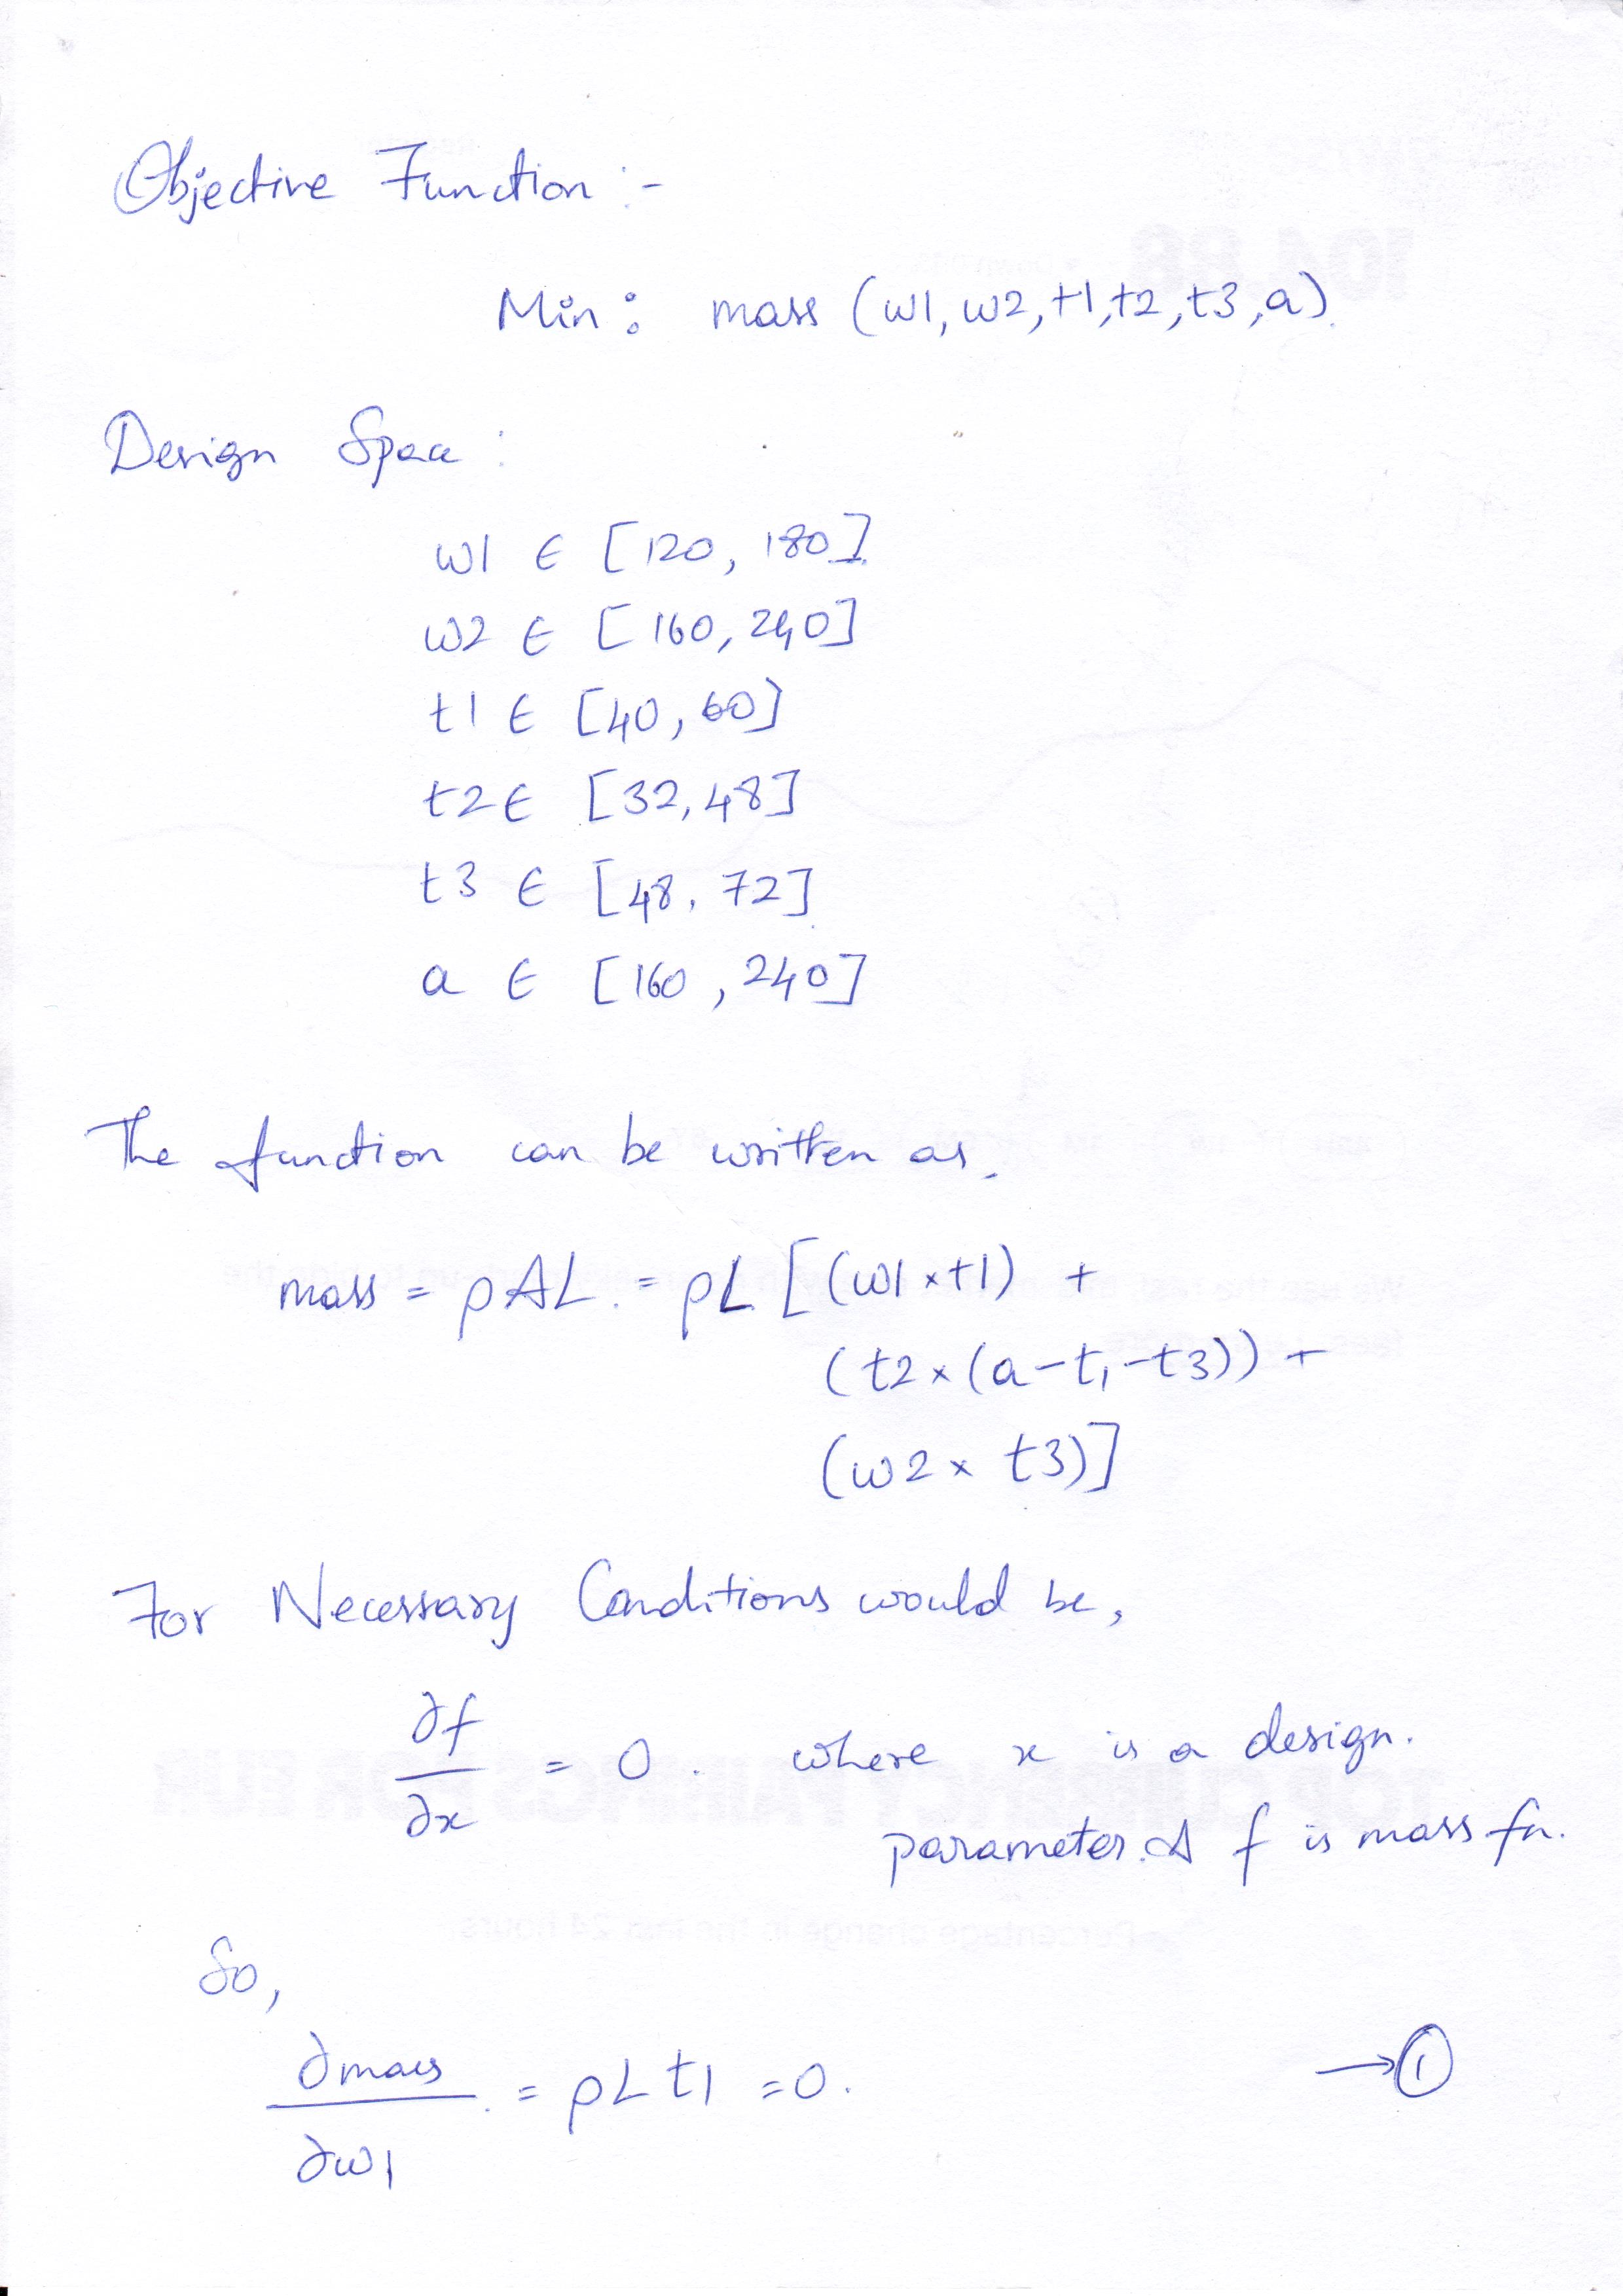
\includegraphics[keepaspectratio]{p1.jpeg}}

\pandocbounded{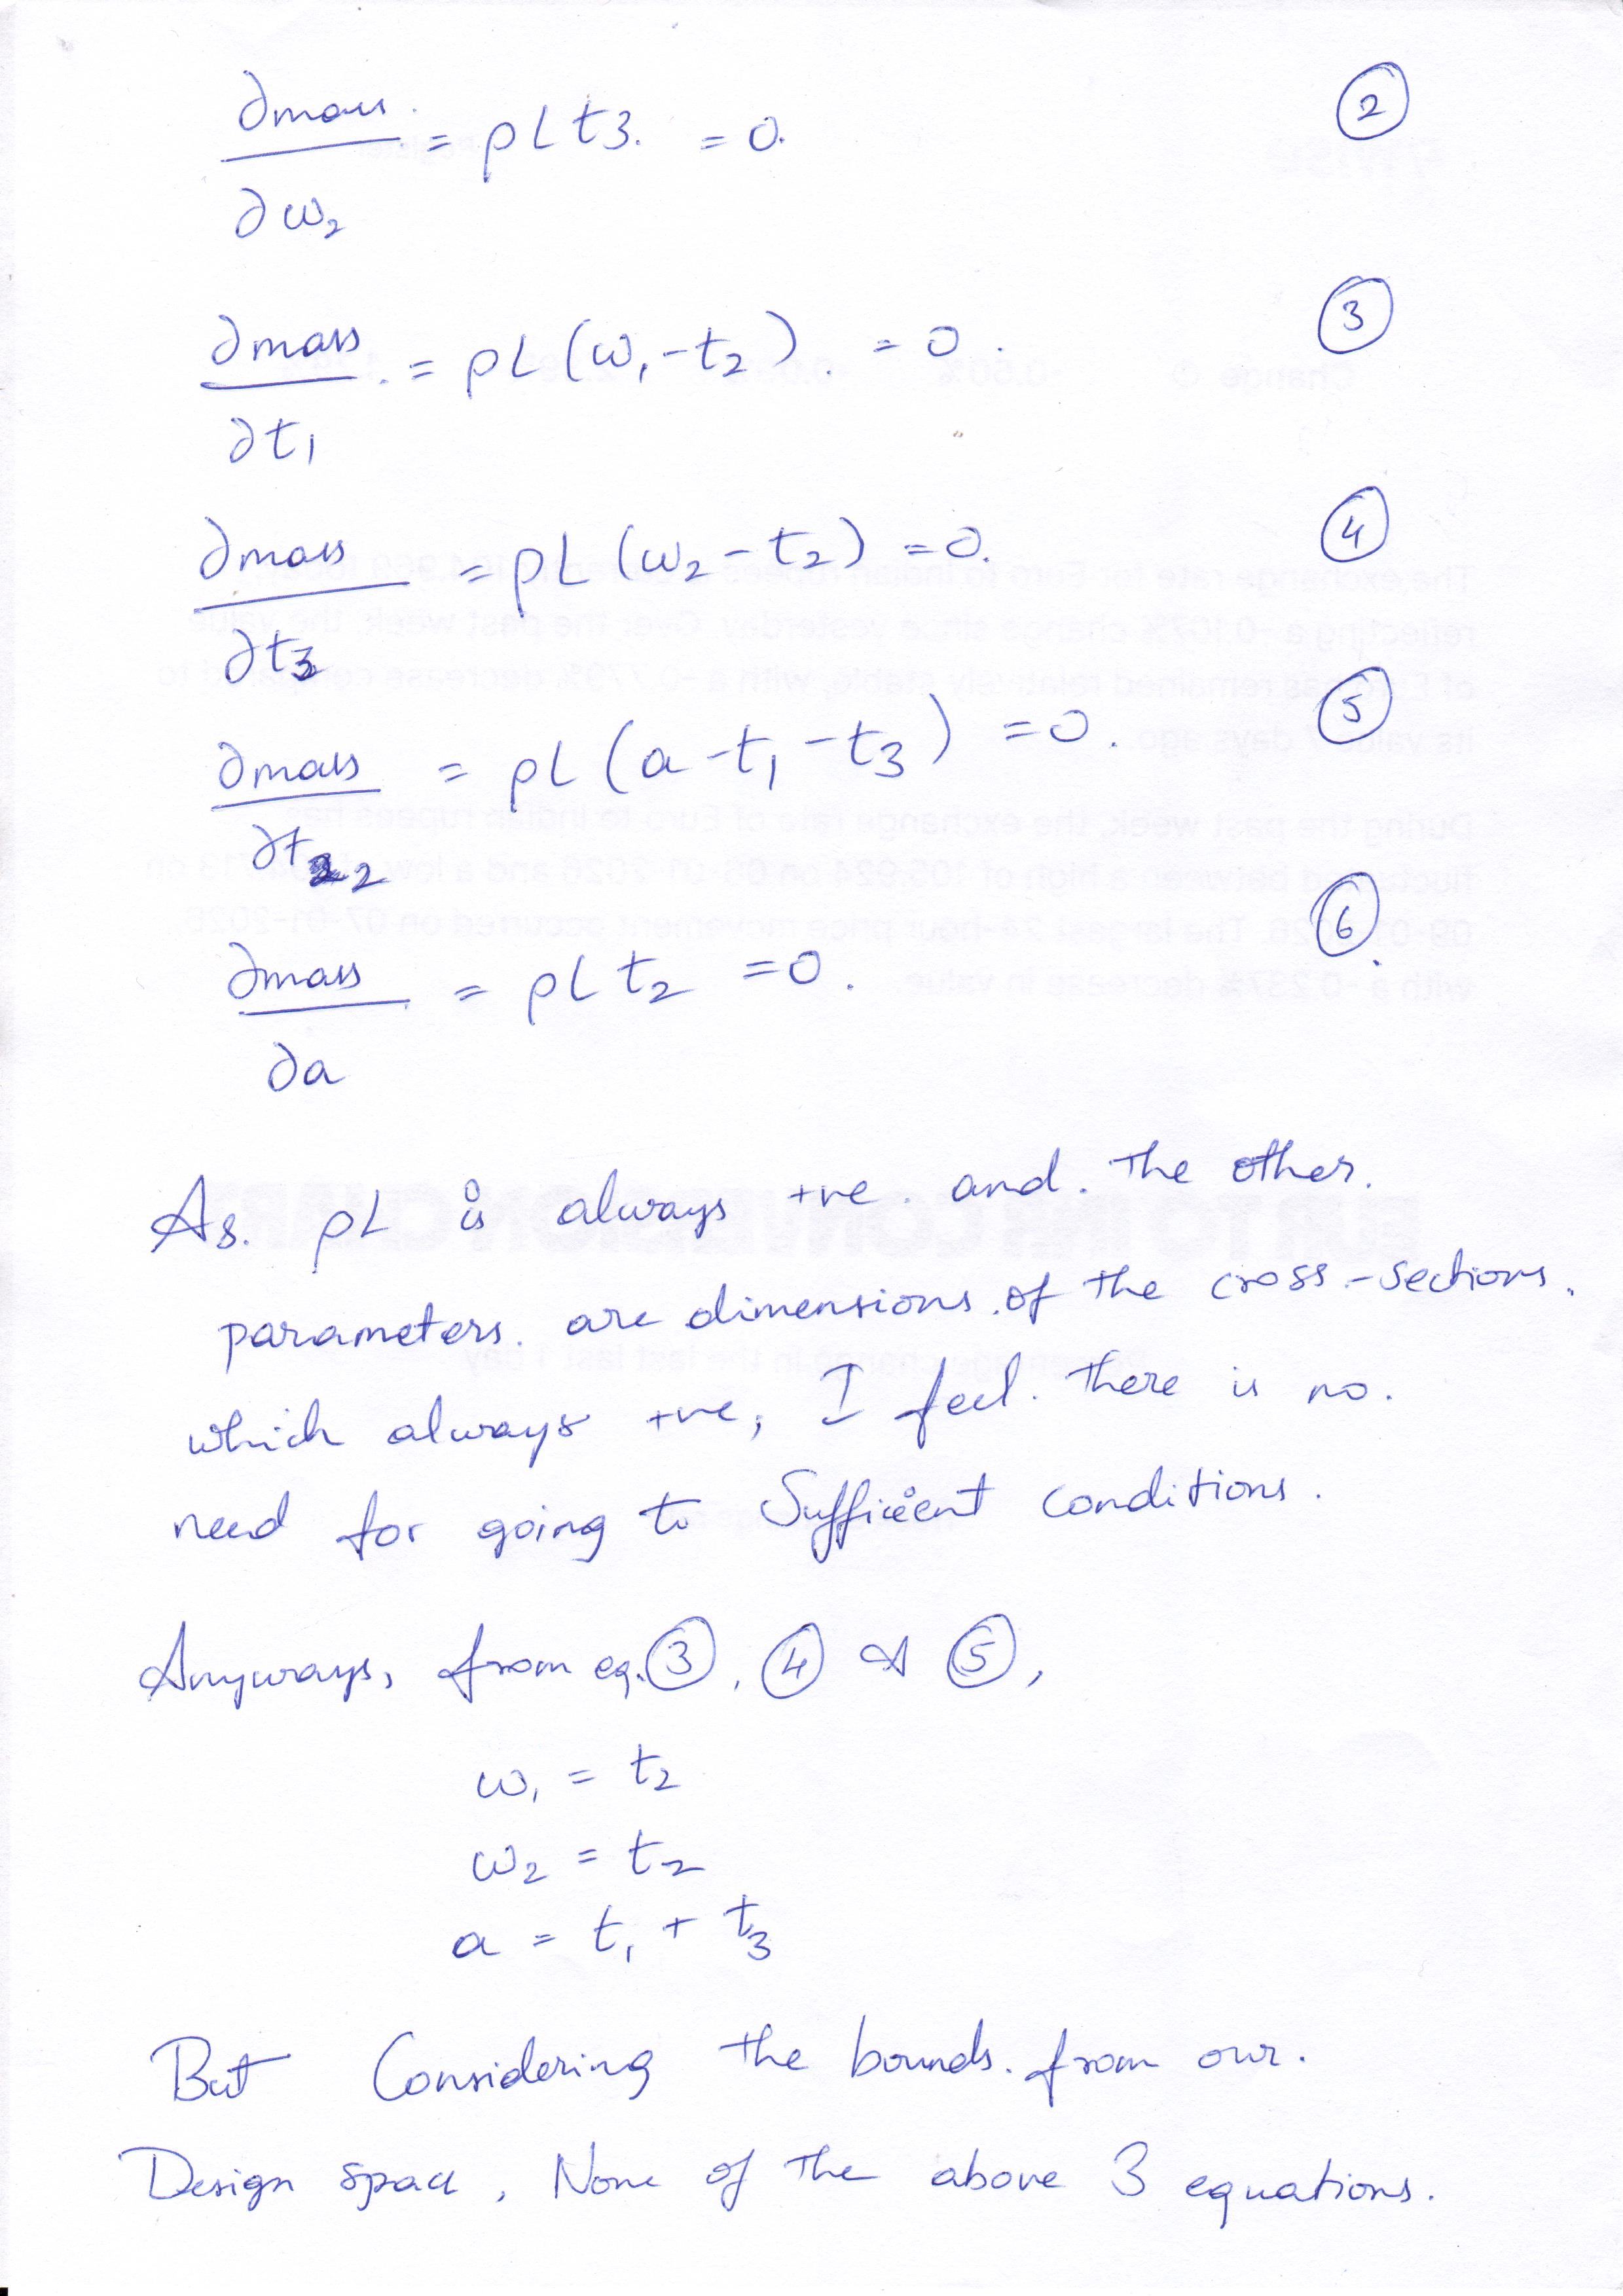
\includegraphics[keepaspectratio]{p2.jpeg}}

\pandocbounded{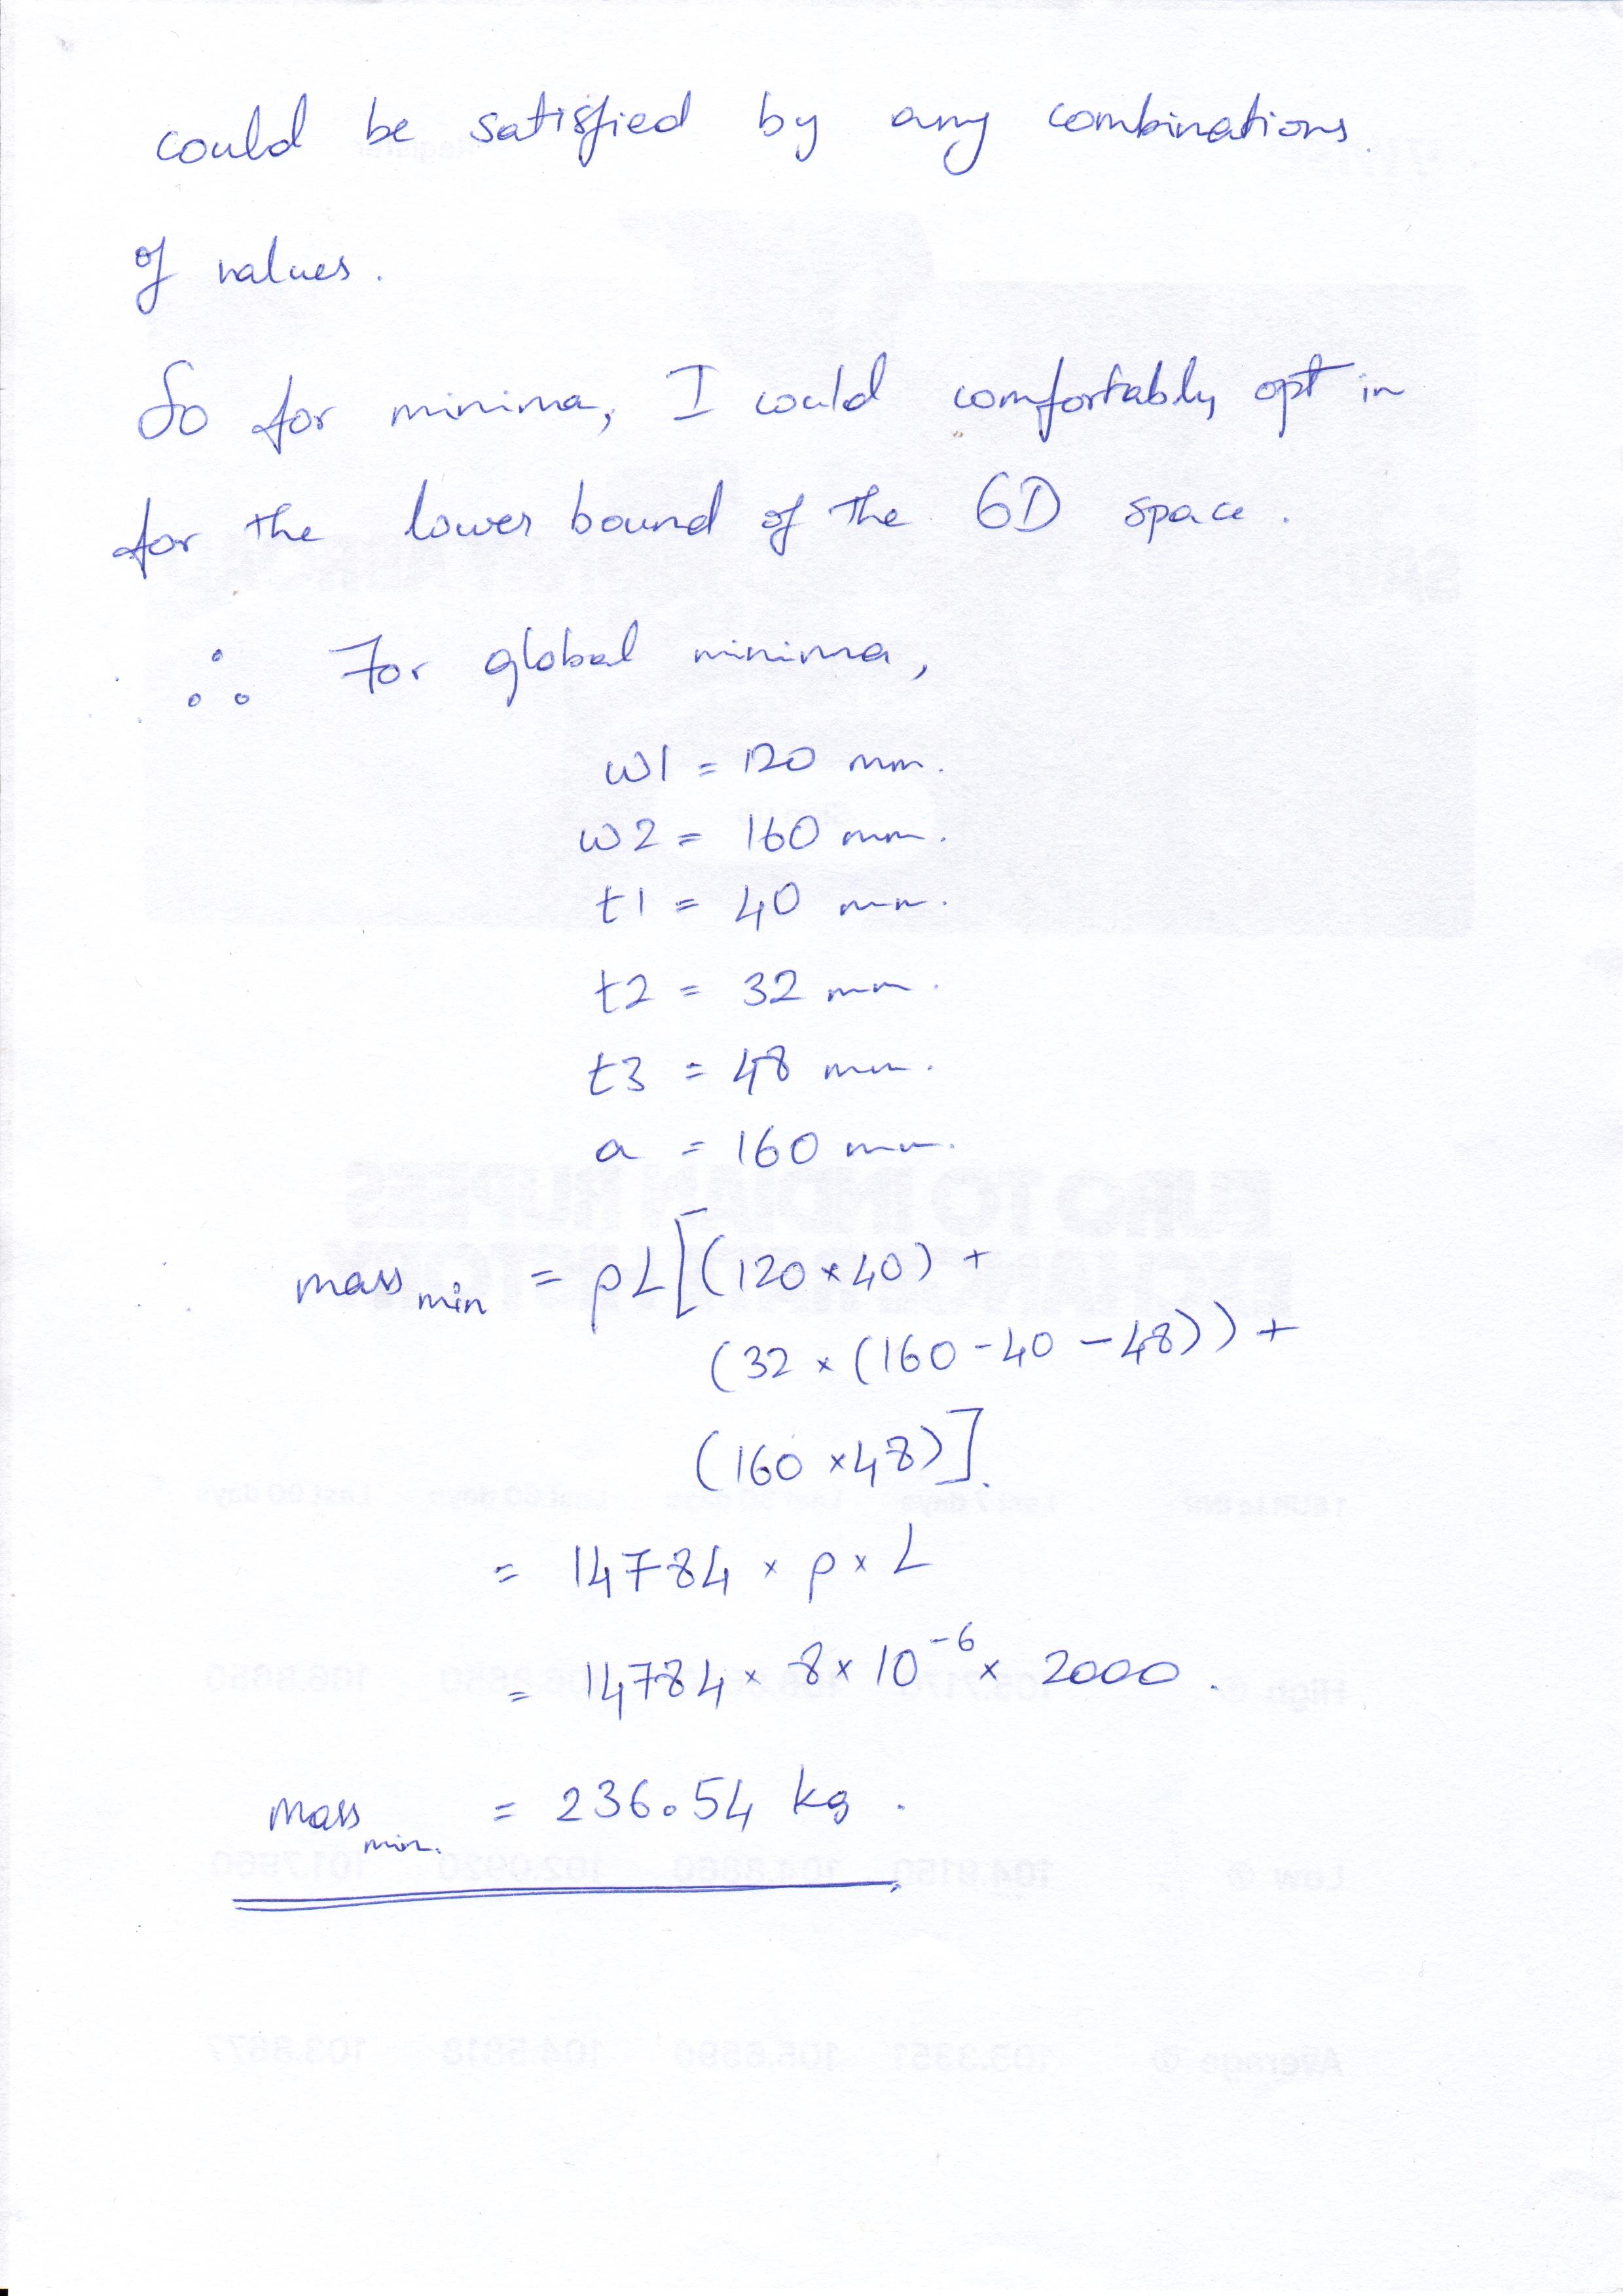
\includegraphics[keepaspectratio]{p3.jpeg}}




\end{document}
